% article example for classicthesis.sty
\documentclass[11pt,a4paper]{scrartcl} % KOMA-Script article 
\usepackage{lipsum}
\usepackage{url}
\usepackage[LabelsAligned]{currvita} % nice cv style
\usepackage[nochapters]{classicthesis} % nochapters
\usepackage{tikz}
\usepackage{amsthm}
\usepackage{setspace}
\usepackage{pifont}
\usepackage{color}
\usepackage{graphicx}
\usetikzlibrary{calc,shapes,arrows,automata,trees,shadows,decorations.pathmorphing,positioning,
shapes.misc,shapes.arrows,chains,matrix,scopes,decorations.pathmorphing,backgrounds}
\renewcommand*{\cvheadingfont}{\LARGE\color{Maroon}}
\renewcommand*{\cvlistheadingfont}{\large}
\renewcommand*{\cvlabelfont}{\qquad}
\DeclareGraphicsExtensions{.pdf,.png,.jpg}
\begin{document}
\pagecolor{Sepia!04}
%Coverletter
\begin{cv}{\spacedallcaps{Title}}
        \begin{cvlist}{\textcolor{brown}{\spacedlowsmallcaps{Jason~N~Mansfield}}}\label{PersDat}  
            \item   Regis University
            \item   3333\\
                    Regis Boulevard Denver \\	
                    Colorado 80221-1099
            \item   mansf843@regis.edu\\				
                    \url{http://www.regis.edu/}				
        \end{cvlist}
        \begin{cvlist}{\spacedlowsmallcaps{RC~471}}\label{irgendwas}
            \item Instructed by Professor~Henri~Tshibambe\\
             \url{http://tinyurl.com/3htorkr}
        \end{cvlist}
    \end{cv}
\clearpage
\noindent
\textcolor{Maroon}{\spacedallcaps{The quoted article title}}\\
\textcolor{brown}{\spacedlowsmallcaps{Philippians~2~\cite{niv}}}
\begin{verse}
6\\ Who, being in very nature God, \\ did not consider equality with God \\ something to be grasped, 
\end{verse}
\begin{verse}
7\\ but made himself nothing,\\ taking the very nature of a\\ servant, \\ being made in human likeness.
\end{verse}
\begin{verse}
8\\ And being found in appearance as\\ a man,\\he humbled himself\\ and became obedient to death —\\ even death on a cross!
\end{verse}
\begin{verse}
9\\ Therefore God exalted him† to the\\ highest place\\ and gave him the name that is above\\ every name,
\end{verse}
\begin{verse}
10\\ that at the name of Jesus every\\ knee should bow,\\ in heaven and on earth and under\\ the earth,
\end{verse}
\begin{verse}
11\\ and every tongue confess that Jesus Christ is Lord,\\ to the glory of God the Father.
\end{verse} 
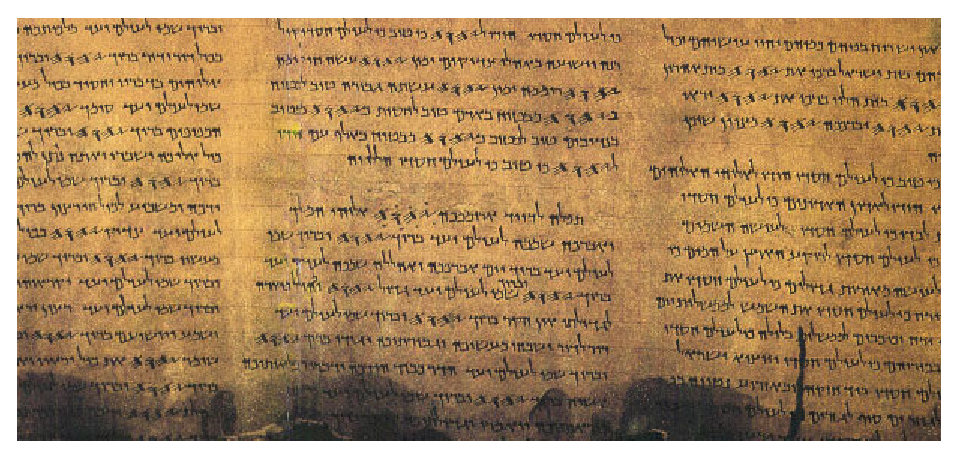
\includegraphics[scale=1]{deadsea}
\clearpage
%Title
\title{\textcolor{Maroon}{\rmfamily\normalfont\spacedallcaps{Title again}}}
    \author{\textcolor{brown}{\spacedlowsmallcaps{Jason N Mansfield}}}
    \date{} % no date
    
    \maketitle
    
    \begin{abstract}
  
    \end{abstract}
       
    \tableofcontents
    
    \section{Childhood}
When I was very young my parents began teaching me to read. I would spend a large portion of my time reading from the bible due to the frequency of our studies. My mother also at an early age would read the bible but did not become a Jehovah's Witness until near her teenage years. My father on the other hand went to more Mainline Protestant type churches and converted later to become a Jehovahs Witness. Die to the rigorous readings each week I could read and write at a very early age as could my younger brother and sister. 

  % bib stuff
    \nocite{*}
    \addtocontents{toc}{\protect\vspace{\beforebibskip}}
    \addcontentsline{toc}{section}{\refname}    
    \bibliographystyle{plain}
    \bibliography{cite}
\end{document}